\chapter{Analysis and Design}
The focus of this chapter is to establish and discuss what is the software going to do, and how is going to achieve its intended goals. The actors in defining this are the stakeholders. The process of doing so is through the requirements elicitation. It is important to mention that  

\section{Users and stakeholders}
As mentioned before, prior to the start of the development phase, it is important to establish who are the intended users of the application, as well as the stakeholders. 

The following users were depicted for this development:

\begin{itemize}
	\item General public: The general public who is concerned whit the air quality of their environment.
    \item Pollution-sensitive public: People at risk of suffering health consequences due to air pollution.
\end{itemize}

In order to gain input from different perspectives, the following stakeholders were involved through the development: 

\begin{itemize}



	\item Researchers 
    \begin{itemize}
      \item Asthma UK researchers: Meetings were arranged with various researchers of the asthma UK group. They were involved early in the design of a first prototype, by providing ideas and highlighting issues that may arise from a medical researcher perspective. The queried researches were:  Dr. Aziz Sheikh, director of the research group, Dr. Soyiri Ireneous, and Dr. Lynn Morrice.
    The following issues were raised in the meetings:
      \begin{itemize}
          \item Applications that rely on user input are not sustainable.
          \item Review past approaches/work to avoid known problems.
          \item An application should give actionable feedback rather than just displaying information.
          \item Ask the users to know what they want.
      \end{itemize}
      \item University of Edinburgh researchers: My supervisor and Cat. Mcgill

	\end{itemize}
    
	\item Domain experts    
   \begin{itemize}
      \item Chief Technology Officer: Simon Chapple acts as chief technology officer of Datalytics technology, a company who has expertise on developing mobile applications for a different range of platforms, his opinion would prove valuable with respect of more technical or design issues that may arise in the development. He was asked for feedback about the design of a prototype of the application.
    The following recommendations were raised in the meeting:
    \begin{itemize}
		\item User interfaces should aim to be self-explanatory. 
		\item Colors should be consistent and provide meaning, as users associate colors to real world entities.
		\item Further consideration should be taken when choosing a native vs hybrid development approach.
		\item Welcome screens should have an immediate, understandable objective.   
	\end{itemize}
	\item How to ref this?: Mic starbuck, an activist who is involved in the guverment council and suffers from asthma was involved in the very first ideas of the design of the application, from his input, we were able to understand in a broad sense, what might an asthma sufferer need.
	\end{itemize}
%"I wonder how you did the animations behave that way"

	\item Users as stakeholders: The final users were involved in three stages, in the requirements elicitation, as co-designers for the prototypes, and as evaluators  of the final product. 
    \begin{itemize}

		    \item The Asthma UK patient group: The patient group of the Asthma UK for applied research was involved in two phases: The requirements elicitation via an online questionnaire, and the evaluation of the final product.
			\item General public: They were involved in three phases: The requirements elicitation via an online questionnaire, the evaluation of  prototypes and the evaluation of the final product. 

	\end{itemize}

\end{itemize}

\section{Requirements elicitation}
According to Somerville \cite{Sommerville2010}:
\begin{displayquote}
\begin{itemize}

\item Functional requirements: statements of services the system should provide, how the system should react to particular inputs, and how the system should behave in particular situations

\item Non functional requirements: Constraints on the services or functions offered by the system.... often apply to the system as a whole, rather than individual system features or services.


\end{itemize}
\end{displayquote}

The main functional requirements were elicited from the users because they were the first reason of the development. This was done through an online survey monkey questionnaire\footnote{\url{https://www.surveymonkey.com/results/SM-Z7HH28LM/}}, the survey was sent to the aforementioned Asthma UK patient group, and to the general public through different survey collectors to be able to compare the responses between them. Feedback from researchers and domain experts was taken into account as non-functional requirements, they did not ask for any function per se. but just established some guidelines and features that would be nice to have in an application. 

\subsection{Survey}

When designing the questionnaire, there was an interest in knowing which existing air quality data sources both kind of users were employing and what did they find useful from those sources, they were also queried regarding on how often they were using the information sources, their ages, and their and their needs towards a new air-quality application.

The total number of responses were 11, 8 of them being from the patient group, and 3 of them from the general public. The ages of the respondents were varied: 3 between 25-34, 3 between 65-74, 2 between 18-24, 2 between 35-44 and one between 55-64 years old as shown in the figure \ref{fig:survey_ages}. 

\begin{figure}[H]
\begin{adjustbox}{width=1\textwidth,center=\textwidth}
  \centering
  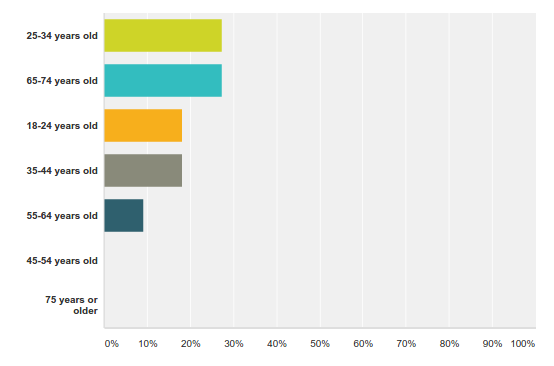
\includegraphics[scale=1]{images/ages_survey.png}
\end{adjustbox}
  \caption[Survey respondents ages ]{Survey respondents ages}
  \label{fig:survey_ages}
\end{figure}

Regarding previous usage of air quality sources, its was shown that only half of the sensitive respondents were able to name the websites or applications they were currently using, while all the non sensitive respondents named at least one source of information. Also, the sensitive respondents who reported the use of air quality sources, tended to use them in a more regular basis than non sensitive users. Reflecting on these answers; sensitive users may be inclined to require a support tool on a regular basis; but not all of them are aware of their existence, or simply does not feel the current sources meet their needs. 

The main findings from the survey were the potential new functionalities that users would like in a new air quality application, they depict that there are undressed needs from current AQ sources. These are the main focus of the development of a new air quality application. From the \ref{fig:survey_new_features} we can see that the most important need is to visualize different individual pollutants, as current approaches (REF as discussed in ) sources often fail to categorize them and indicate what might they be affecting towards a person's health. The second most important undressed need is to be able to personalize the air quality advice given their personal circumstances; and the third most important requirement is to compare and visualize individual pollutants over different periods of time. Another interesting outcome of this question was if including tools that would allow the users to keep track of their symptoms would be of interest; but just three of the eleven queried persons responded this is the case. Response later supported from researchers in the health field based on their experiences. 


\begin{figure}[H]
\begin{adjustbox}{width=1\textwidth,center=\textwidth}
  \centering
  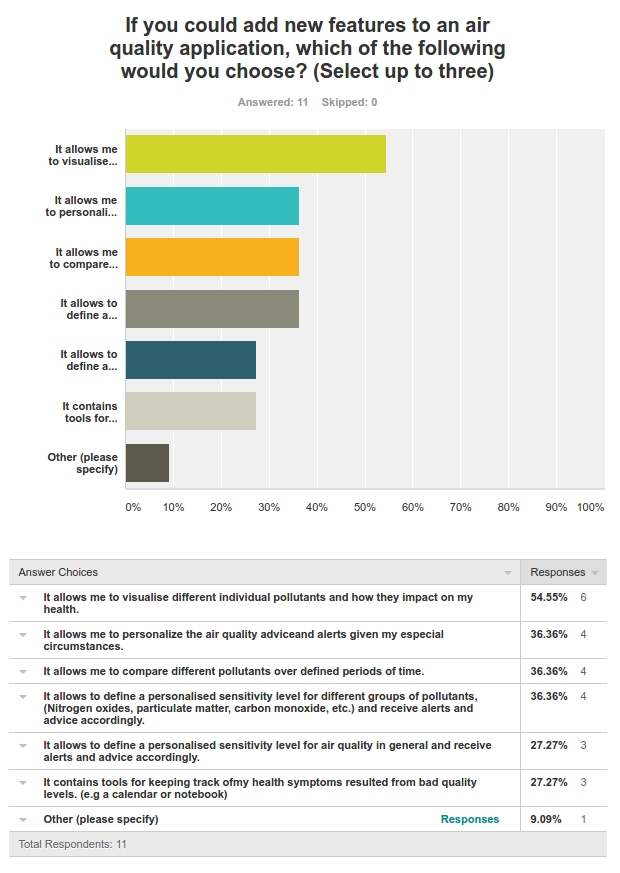
\includegraphics[scale=1]{images/new_features.png}
\end{adjustbox}
  \caption[New features for an AQ application]{New features for an AQ application}
  \label{fig:survey_new_features}
\end{figure}

\subsection{Interviews}

Meetings were held with the aforementioned researchers and domain experts to receive input from different points of view. At early stages of the design, the first person who showed interest was Mic. Starbuck. From his perspective as a person suffering from asthma; he mentioned the need of a tool to be able to visualize the relative impact upon a person's health given different factors: like a person's health status, location, altitude, and specific pollution particles. He mentioned as well that he browsed the web frequently to understand how the AQ was behaving at different points of the day in order to decide whether or not going outside or perform certain activities. 

Later on, the Asthma UK center for applied research showed interest and a meeting was arranged. It took place with Dr. Aziz Sheikh, Moyrrice Lynn, Dr. Soyiri Ireneous and Cat. Mcgill. They showed a favorable interest on collaborating with this project as well as participating closely to the School of Informatics in future research. They were presented with mock-ups as ideas for an application that would accomplish visualization and tracking purposes. However based on previous work on tracking asthma status; they pointed out that applications that rely on user input are not sustainable; as they have to account for more factors, such as the person's age, health issues, and the ability to remember recording the events; and recording them correctly. 

Another meeting was held with Dr. Soyiri Ireneous who's main research is on asthma, and Cat. Mcgill as , the purpose of this meeting was to understand more in-depth the consequences of air pollution upon a person's health and how they might be presented in an air quality application. The possibility to include a health advice was discussed, and he brought up the issue of giving health feedback that can be accounted at the moment of a contingency. Also, Dr. Soyiri as a mobile phone user was concerned is concerned with the speed of the applications he installs, as well the memory and battery usage.


\subsection{Functional requirements}

Because the time is limited; the development will try to cover the first three and most important needs given by the final users as illustrated in the past section. The following list summarizes the final formal functional requirements for the development:

\begin{itemize}
	\item Being able to visualize the air quality status in general.
	\item Being able to visualize individual pollution particles status.
	\item Being able to visualize the impact of pollution particles on a person's health.
	\item Being able to visualize individual pollution particles over time.
    \item Being able to receive actionable health advice.
    \item Being able to personalize the received health advice.
\end{itemize}

\subsection{Non functional requirements}

Summarizing from the meetings, the following was established as non functional requirements:

\begin{itemize}
	\item Should be adequate for mobility (\textbf{Mobility}).
	\begin{itemize}
		\item Not consume much storage space.
		\item Not consume much battery.
	\end{itemize}
    \item Should be usable (\textbf{Usability}):
    \begin{itemize}
		\item Easy to learn.
        \item Attractive to use.
	\end{itemize}
    \item Should be efficient (\textbf{Performance}).
    \begin{itemize}
		\item Start rapidly
        \item Load and display visualizations fast
	\end{itemize}
    
\end{itemize}


\section{System architecture}
In order to accomplish the requirements, it is important to consider design choices that could add towards qualities that are more adequate for this kind of development. For this, a trade-off between the three main qualities for the software will be considered as shown in Figure \ref{fig:balance_attributes}, as it is not always possible to have everything in a system because some attributes may contradict between each other. For example, doing an extremely animated and attractive design would affect the performance of the system and its capability to accomplish the main goal. Architectural choices will be taking into account this trade-off.


\begin{figure}[H]
\begin{adjustbox}{width=.5\textwidth,center=\textwidth}
  \centering
  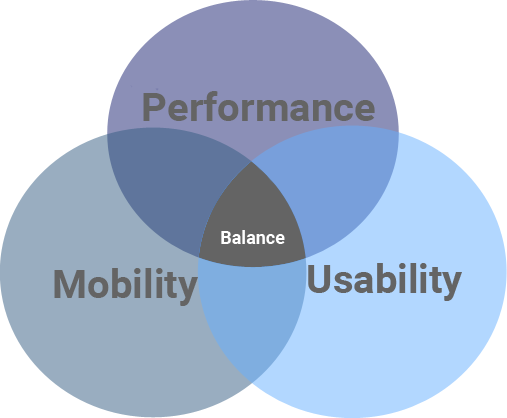
\includegraphics[scale=1]{images/balanceCircles.png}
\end{adjustbox}
  \caption[Finding a balance between software attributes]{Finding a balance between software attributes}
  \label{fig:balance_attributes}
\end{figure}

\subsection{Development approach and operative system}
It is possible that the development could take a hybrid or a native approach, as summarized in the table \ref{tab:development_approaches}. In a nutshell, it means that the software could be developed in a web-browser container and therefore be compatible with all devices, or be developed using the native software development kit for each system (Android, iOS, etc); being only compatible with that specific operative system. A native development approach carries the disadvantage that new code would be needed for each operative system; but gaining many benefits, such as the response speed, being able to use advanced graphics and animation techinques; and having an easy access to the native APIS and components of the device (Such GPS or gyroscpe). In order to gain performance and usability a native approach has been chosen. Following it is important to define the operative system target, which will solely based on the market share of the most important operative systems according to IDC \footnote{\url{http://www.idc.com/prodserv/smartphone-os-market-share.jsp}} . Android keeps an enormous share of 82.8\% compared to a 13.9\% of iOS, and a 2.6\% of Windows phone (other systems just account for less than 1 percent of the market share.) 
(Android version)

\begin{table}[ht]
\centering
\begin{adjustbox}{width=.6\textwidth,center=\textwidth}
\begin{tabular}{lrr}
  \hline
   - & Native & Hybrid  \\ \hline
   Language & Switf or Java & HTML and Javascript \\
   Speed & Fast & Medium \\
   Portability & None & High \\
   Advanced Graphics & High & Moderate \\
   Access to native APIs & High & Moderate \\
   Development cost & Expensive & Reasonable \\
   \hline
\end{tabular}
\end{adjustbox}
  \caption[Native vs hybrid development approach ]{Native vs hybrid development approach. (Adapted) \footnotemark }
\label{tab:development_approaches}
\end{table} 
\footnotetext{\url{http://julyrapid.com/hybrid-vs-native-mobile-app-decide-5-minutes/}}

\subsection{Air quality data source}
It was considered to acquire personal air quality sensors to provide real-time high resolution data to the system; unfortunately, such devices are still not very feasible as they are costly and become disposable over time due its loose of accuracy. One example is the Libelium gases pro sensor, which costs around \euro{}2000 and has an approximate lifetime of 12 months\footnote{\url{http://www.libelium.com/calibrated-air-quality-gas-dust-particle-matter-pm10-smart-cities/}}. 

As mentioned in section (REF) there are currently many fixed sensors around Scotland. Which include different measures depending on the type of the sensor; however, the data sensed with this devices is not exposed through any public API from the Scottish government. But just as plain HTML information trough DEFRA websites (REF). One possibility as well is use any third party air quality data source; such as the breezometer air quality API\footnote{\url{https://breezometer.com/air-quality-api/overview/}} or the OpenAQ API\footnote{\url{https://openaq.org/#/}}. The first one is a private source of air quality data which bills for the queries to the service and may become not very cost-effective, the second is a public API source, but the number of sensors from each city in Scotland are limited compared to the official government sources. An example of this is the city of Glasgow, which from the official sources has 26 fixed sensors and from the public API only 4 are available. Because of this, to have a more accurate air quality source the data will be collected from the official sources and exposed to later query from the device. 

Missing this: (REF)
http://www.scottishairquality.co.uk/data/

\subsection{Infrastructure as a service}
IaaS or Infrastructure as a service is a cloud service that provides computing infrastructure on demand. The benefits of using such service as opposed to a traditional approaches are various. First, there is no need to buy, install and maintain a server on a fixed location, reducing the associated costs. Second, setting up an IaaS can be done within minutes, saving precious development time. The following options were considered for setting up an IaaS: 

\begin{itemize}
	\item Google Cloud platform \footnote{\url{https://cloud.google.com/}}
    \item Amazon Web Services \footnote{\url{https://aws.amazon.com/}}
    \item Microsoft Azure \footnote{\url{https://azure.microsoft.com/en-us/}}
\end{itemize}

Because of budget constraints, the most cost-effective solution was chosen, being Amazon's free tier the most generous allowing up to 12 month of free usage, as opposed to Microsoft's 30 days trial and Google's 60 days trial.

\subsection{Back-end technological choices}
The back end component of the system will perform 2 functions. Gather the required air quality data and insert it into a database; and provide service to the mobile application. For the  first function; the easiest way to do it is via any available web-crawling libraries, such as Jspider\footnote{\url{http://j-spider.sourceforge.net/}} for Java or Scrapy \footnote{\url{http://scrapy.org/}} for Python. Scrapy was chosen because it is a complete and stable framework that can handle the crawling operations in an easy way. 
For the second component; there is a need for a more robust component which can handle multiple queries to the health advice presented in Android. Because of this, Java will be 

\subsection{Schema-free database}
There will be the need to store the air quality readings somewhere to later query from the device. For this, there is the option to use standard SQL databases or schema-free databases. Analyzing the data that will be stored in further detail; it will contain the readings gathered from each sensor in Scotland, and specific information such as their name, location and type of sensor, simple enough to be inserted without any relational schema . Moreover, the transactions between the devices and the database should be as fast as possible; without caring to much for instant reliability (because the sensors are updated at the soonest each hour). Taking into account these factors, it is more suitable the usage of a schema free database or NoSQL, specifically, it will be used a Dynamo NoSQL from the same Amazon Web Services infrastructure because it integrates easily with the already chosen IaaS. 

\subsection{Amazon web services SDK}
The easiest way to communicate between the Android device and the services provided by amazon is by using the SDK provided by Amazon\footnote{https://aws.amazon.com/mobile/sdk/}, 

\subsection{Overall design}
The overall design of the infrastructure will be as shown in Figure \ref{fig:architecture}. The back-end and the database components will be running in amazon web services, and the android device will make use of the AWS SDK to make queries to the dynamo database; and REST services to query the advice server running on Java.

\begin{figure}[H]
\begin{adjustbox}{width=.8\textwidth,center=\textwidth}
  \centering
  \includegraphics[scale=1]{images/architecture.png}
\end{adjustbox}
  \caption[Architecture design]{Architecture design}
  \label{fig:architecture}
\end{figure}

\section{Mobile application}
The Android application will be the visible interface for the final user. At this point it is pertinent to understand the design choices that can affect towards our main quality attributes: the design of the user interface, and the lower-level issues related to the management of the screen components. 

\subsection{User interface}
Three distinct screens will accomplish the functional requirements as shown in Figure \ref{fig:chain_of_screens}. The first screen will be responsible for displaying a general overview and the personalized advice, the second screen will show individual pollutants; and the third screen will show individual pollutants over time. 

One useful guideline at design level in order to connect the screen between each other is simplicity. Having many different screens that accomplish many different purposes could result in overwhelming the user, because of this, the screens will be accessible at every time using a tabbed menu and enabling gestures to navigate through them. That is, the screens will become active by selecting a tab, or by swiping between the screens. 

\begin{figure}[H]
\begin{adjustbox}{width=.45\textwidth,center=\textwidth}
  \centering
  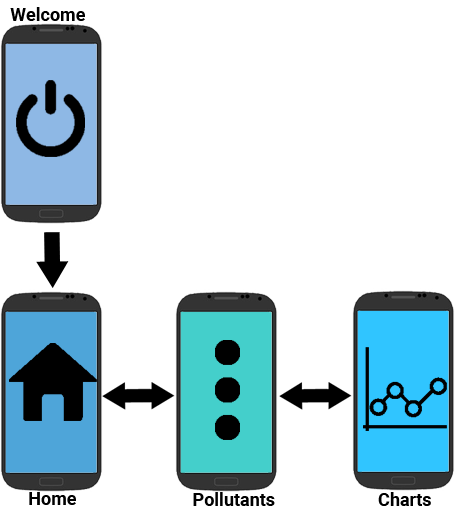
\includegraphics[scale=1]{images/screenChain.png}
\end{adjustbox}
  \caption[Chain of screens]{Chain of screens}
  \label{fig:chain_of_screens}
\end{figure}

\subsection{Activities}
The former screens will be developed individually by the use of activities. An activity is the abstraction used by the Android framework to contain the visual and run-time elements of the current displayed screen. The way activities are created and maintained in the screen is quite unusual in contrast with standard Java Swing interfaces. It makes use of an event driven life-cycle that must be understood ahead in order to achieve an smooth and error-free behavior. 

Because the available RAM is limited in a handled device and it has to be shared with all other running applications, it is not possible to maintain  all activities instances in memory. The activities lifecycle is a workaround for this problem, allowing the dalvik virtual machine (A virtual machine that runs all Android programs) to automatically handle which activities will be kept on memory. Therefore, it is unknown the time it will be requested to start-up resume or stop and all possible precautions should be taken for it to keep working from any call point .

The lifecycle is illustrated in Figure \ref{fig:activities_lifecycle}, it can be observed that the first method called by Android is the \textit{onCreate()} method, used to instantiate the requested activity and any screen components. Later on, the application can pass to other states until it is stopped and started again from a different entry point to the one it was previously created from. The activities should be able to handle both starting points and restore any state left by the user when the activity was requested to stop. 

\begin{figure}[H]
\begin{adjustbox}{width=1\textwidth,center=\textwidth}
  \centering
  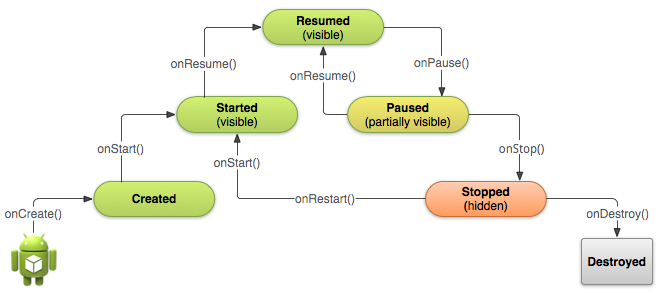
\includegraphics[scale=1]{images/basic-lifecycle.png}
\end{adjustbox}
  \caption[Android activities lifecycle]{Android activities lifecycle\footnotemark}
  \label{fig:activities_lifecycle}
\end{figure}
\footnotetext{\url{https://developer.android.com/training/basics/activity-lifecycle/starting.html}}

\subsection{Layouts}
The main component to render a screen in Android is the Layout. Layouts make use of XML to define the objects in the screen as shown in the example bellow, which renders a \textit{TextView} object followed by a \textit{Button} object. Layouts need to be attached to an activity or fragment to give them behavior. Once attached, the components defined by the layout can be extracted by using their id's and the method \textit{findViewByID}

\begin{verbatim}
<?xml version="1.0" encoding="utf-8"?>
<LinearLayout xmlns:android="http://schemas.android.com/apk/res/android"
              android:layout_width="match_parent"
              android:layout_height="match_parent"
              android:orientation="vertical" >
    <TextView android:id="@+id/text"
              android:layout_width="wrap_content"
              android:layout_height="wrap_content"
              android:text="Text" />
    <Button android:id="@+id/button"
            android:layout_width="wrap_content"
            android:layout_height="wrap_content"
            android:text="Text" />
</LinearLayout>
\end{verbatim}

It is important to understand the correct coupling of Android layouts because this influences how fast the screen is rendered. The rendering process is called \textit{inflating} and occurs in the \textit{onCreate()} method. As the activities are rendered on the screen; children components are attached and may call to render their own layout and so on, potentially languishing the the application. For this purpose, the android SDK makes available the Android device monitor that can be employed to understand how much time is taking to render all the components displayed at a given time. 

The Android device monitor helps to visualize the components that are taking part of the screen at some point in run-time. It shows from the top most element (the root) to the bottom most element (the leafes), how they are attached together and which element of the entire tree is taking the most time to render helping in the debugging process. As shown in figure \ref{fig:android_device_monitor} the delaying components are marked with red dots; wich means that the rendering of that specific screen component is among the slowest half of views, the yellow means the view renders faster than the bottom half of the other views and the green means that renders faster than at least half of the other views. The understanding of this tool is important in order to achieve the required performance quality attribute. 

\begin{figure}[H]
\begin{adjustbox}{width=1\textwidth,center=\textwidth}
  \centering
  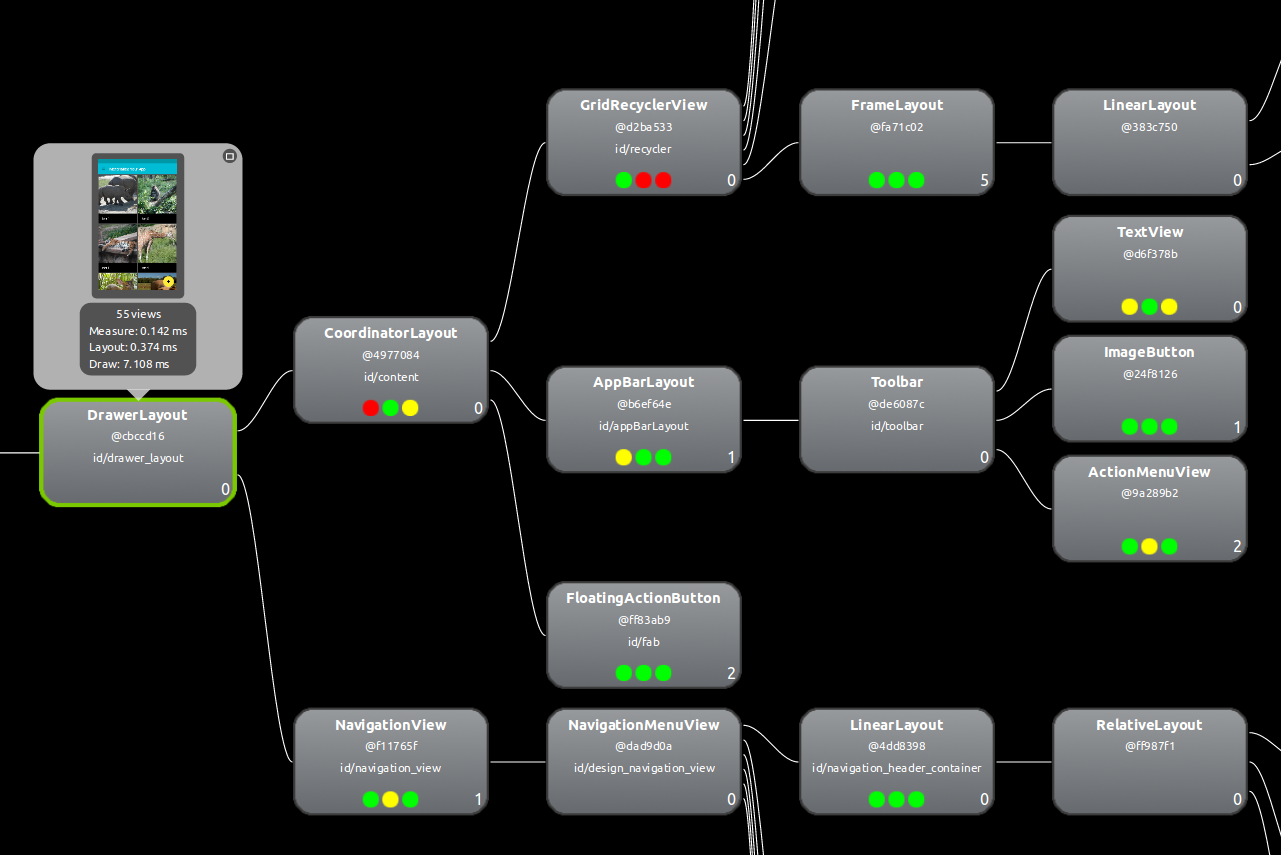
\includegraphics[scale=1]{images/android_device_monitor_2.png}
\end{adjustbox}
  \caption[Andrroid activities lifecycle]{Android device monitor}
  \label{fig:android_device_monitor}
\end{figure}

\subsection{Material design}
As well as understanding how to achieve an smooth behavior within the application is wise to revise how to make good use of the design principles available to enhance usability and its implied attributes: ease of use and attractiveness. 

According to Google: \begin{displayquote}Material design is  a visual language for our users that synthesizes the classic principles of good design with the innovation and possibility of technology and science \end{displayquote} 

The material design framework helps with principles that address design issues to allow every application user to navigate, understand and use the designed user interface (UI) successfully. It also serves to unify the experience across different devices and screen sizes, so that users that are used to applications in general; will be able to understand in a natural way design cues of new applications. The following principles are adhered:   

\begin{itemize}
	\item Material: The material metaphor is based on paper and ink as in the real world, in three dimensions using lights and shadows. The intention is to close the gap between the perception of real world elements and digital elements. 
    \item Graphics: The use of graphical elements such as typographies, icons, adequate colors and images make up a pleasant interface and give hierarchy and meaning. 
    \item Motion: User actions that initiate motion and transform the state of the interface serve as playful cues that help to understand the flow of the interface as well as to provide continuity and feedback. 
\end{itemize}


\begin{figure}[H]
\begin{adjustbox}{width=1\textwidth,center=\textwidth}
  \centering
  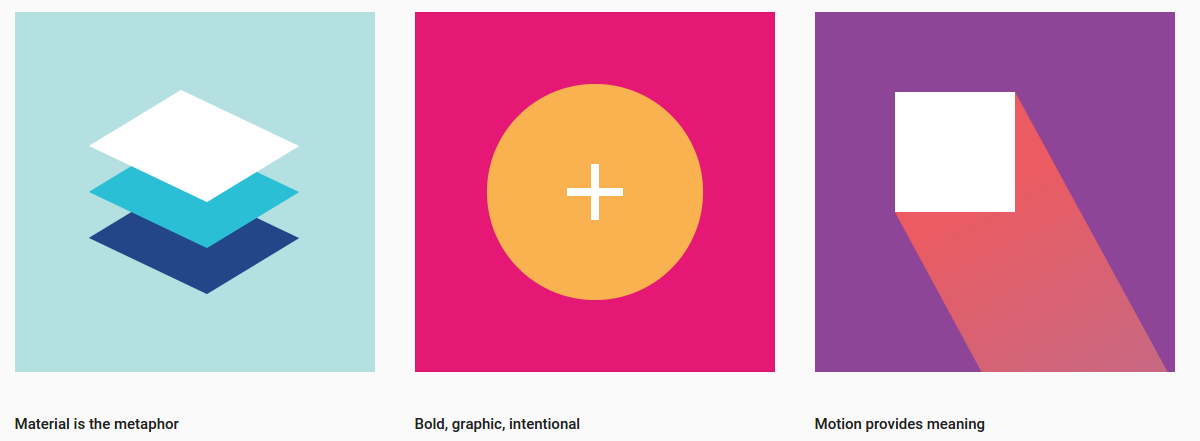
\includegraphics[scale=1]{images/material_google.png}
\end{adjustbox}
  \caption[Material design framework]{Material design framework \footnotemark}
  \label{fig:android_material_design}
\end{figure}
\footnotetext{\url{https://material.google.com/}}

\subsection{Targeted devices}
As the android OS and APIs (Aplication Programming Interfaces) are updated over time; some applications built with later SDK's versions will not be compatible with earlier OS' versions. Because of this, it is important to define the earliest operative system that will be included in the development. For this, considerations such as the number of users that are still using old versions of android and new features that might be useful from newer SDK versions should be considered. For instance, the most used OS distribution nowadays is KitKat which makes use of an API level 19 as shown in Figure \ref{fig:android_platform_versions}, unfortunately, it does not offer native support for material elements, which are a strong positive for this development. A workaround for this problem is to include the Android support library\footnote{\url{https://developer.android.com/topic/libraries/support-library/index.html}} which will provide compatibility for features made available in newer versions of Android. The final targeted API is level 19 (KitKat) to use an up to date stable API and to include up to the 79\% of the Android users.  

\begin{figure}[H]
\begin{adjustbox}{width=1\textwidth,center=\textwidth}
  \centering
  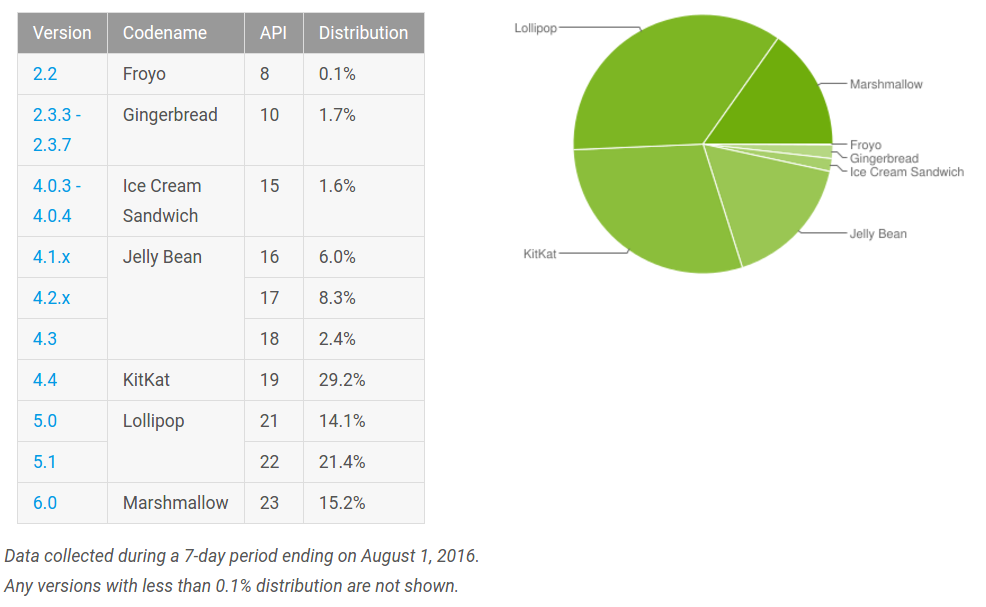
\includegraphics[scale=1]{images/android_platform_versions.png}
\end{adjustbox}
  \caption[Android platform versions distribution]{Android platform versions distribution \footnotemark}
  \label{fig:android_platform_versions}
\end{figure}
\footnotetext{\url{https://developer.android.com/about/dashboards/index.html}}

\section{Back-end}
More in detail, the back-end architecture will be composed as shown in Figure \ref{fig:architecture_back_end_detail}. A virtual machine will run Ubuntu Linux because it is a very stable and compatible version of Linux, there was also a possibility to use a custom amazon flavor of Linux, which was not viable due software compatibility issues. The back-end will host two main components to power the application, the data service and the advice service. 

\begin{figure}[H]
\begin{adjustbox}{width=1\textwidth,center=\textwidth}
  \centering
  \includegraphics[scale=1]{images/architecture_back_end_detail.png}
\end{adjustbox}
  \caption[Back-end architecture]{Back-end architecture detail}
  \label{fig:architecture_back_end_detail}
\end{figure}


\subsection{Data Service}

 The air data source is the air quality in Scotland website. Because the service displays the updated readings in HTML, a web crawler is needed to navigate the readings making use of XPATH selectors to extract the required data. Once extracted, they will be inserted in JSON format directly to the dynamo database.
 
A daemon is a program that runs in the background autonomously, this daemon will call the web crawler every half hour to get the most up-to date readings from the air quality readings (They are updated at most each hour). 

\subsection{Advice Service}
The advice service will be responsible to provide health advice based on the CMEAP\cite{HealthProtectionAgencyfortheCommitteeontheMedicalEffectsofAirPollutants2011}. Before analyzing the techniques that can be considered to translate the advice from the CMEAP into a service, there are few things to notice. The document has different categories of advice based on the sensitivity and age of the persons, they are not simple data statements that can be easily used from a database, but more of simple logical statements. Also, it is likely that the health statements would need to be modified or expanded in the future. 

When it comes to provide logic or 'intelligence' to a system in order for it to take choices (like the ones that are needed for the health advice) there are two general approaches that may be taken. Rule based systems and machine learning techniques. Rule based systems or expert systems are a good fit when all the options for the system are known beforehand; and when all the conditions can be easily written as \textit{if else statements}. On the other hand; machine learning techniques are useful when the datasets are fairly large and the rules have to be made at execution time. Because of this, the easiest way to provide the system the system the capability to give the required health advice given the user's personal circumstances is via an expert system.

\subsection{REST services}
(PEND)

\section{First prototype}
Following the sketched application design and the interaction design methodology, the first prototype was drawn in order to accomplish the user requirements and to start defining how the final interface would look like. As mentioned, the application would be composed of three final distinct visualizations that will achieve the main functional requirements:

\begin{itemize}
	\item Visualize current air quality and provide health advice.
    \item Visualize individual pollutants status and information about their sources and effects.
    \item Visualize individual pollutants over time.
\end{itemize}

The first visualization would contain firsthand pertinent information that would accomplish different functions: letting know in an understandable, visual way the current air quality status and its components, providing information about the source of the air quality reading, showing the air quality advice given the user configuration and let the user configure the air quality advice in a playful way. We could think of this screen as a dashboard that will give the user the required basic information to use the rest of the application, in fact; the displayed by this screen is enough to get a full picture of what is going on without much detail.

This screen is composed as shown in Figure \ref{fig:first_visualization}. It is visually divided into the top and bottom component. The top component is information about the sensor to provide the user confidence about the reading by means of a map, the hour it was last updated, and the name location of the sensor. The bottom component contains two bars: one for adjusting the sensitivity level, and the other one to show the air quality status followed by the advice and the pollutants that are taking part of the reading at the point it was taken. 
\begin{figure}[H]
\begin{adjustbox}{width=1\textwidth,center=\textwidth}
  \centering
  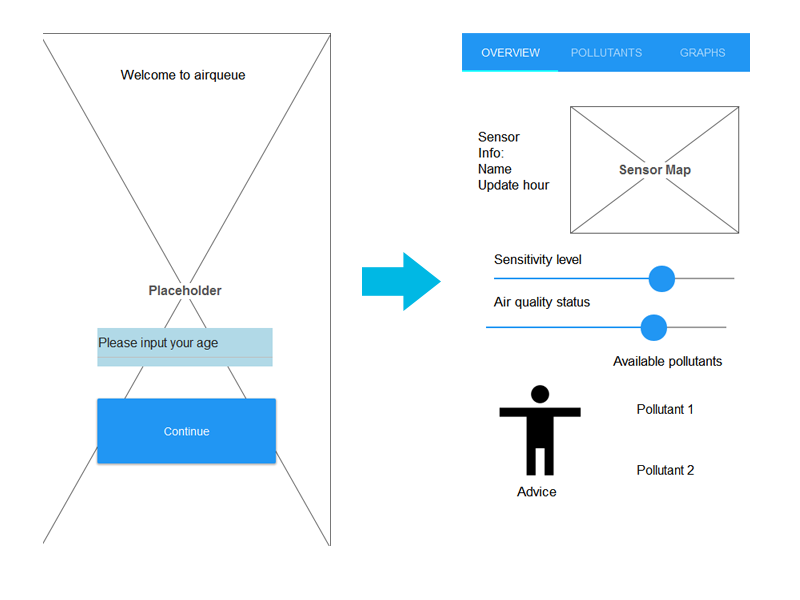
\includegraphics[scale=1]{images/prototype1_screen1.png}
\end{adjustbox}
  \caption[Vsualization 1 first prototype]{Visualization 1 first prototype}
  \label{fig:first_visualization}
\end{figure}

The second visualizations aims to provide an individual visual hint for each pollutant. The need for this visualization arises from the difficulty to observe at a pollutant level how the readings are without expert understanding of the air quality regulations. The overall idea is to show a list of the pollutants that are present at the moment with a visual cue to allow an immediate insight of the reading as well as containing the official measure and the measurement unit. Also, by clicking in each pollutant it will be possible to examine more specific information about the pollutant  

\begin{figure}[H]
\begin{adjustbox}{width=1\textwidth,center=\textwidth}
  \centering
  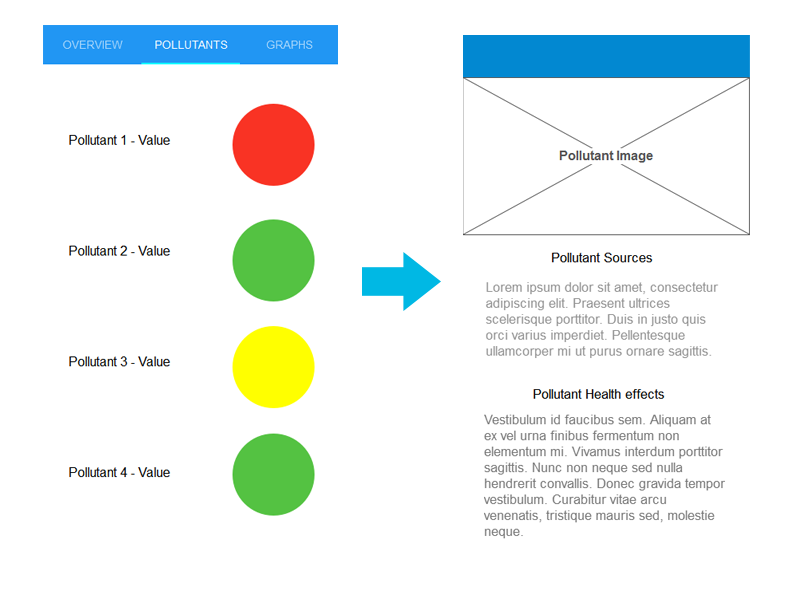
\includegraphics[scale=1]{images/prototype1_screen2.png}
\end{adjustbox}
  \caption[Second screen prototype]{Second screen prototype}
  \label{fig:android_material_design}
\end{figure}

The final visualization will provide the full detail of how the readings were behaving through the day, or in a specific date. The need for this visualization arose from the need by sensitive persons to relate their symptoms to pollution spikes in order to gain knowledge about what might be affecting them at a pollutant level and enable them for better decision support based on this knowledge. For this purpose, a line graph is employed as is the most adequate tool to show readings over time. Also, the same pollutants that were taking part of the first and second visualizations will be consistent in this screen. The difference is that they will be touch-enabled to allow the user to select which  pollutant to visualize. At the top of the screen will be located a button to select pollution data from other dates. 

\begin{figure}[H]
\begin{adjustbox}{width=1\textwidth,center=\textwidth}
  \centering
  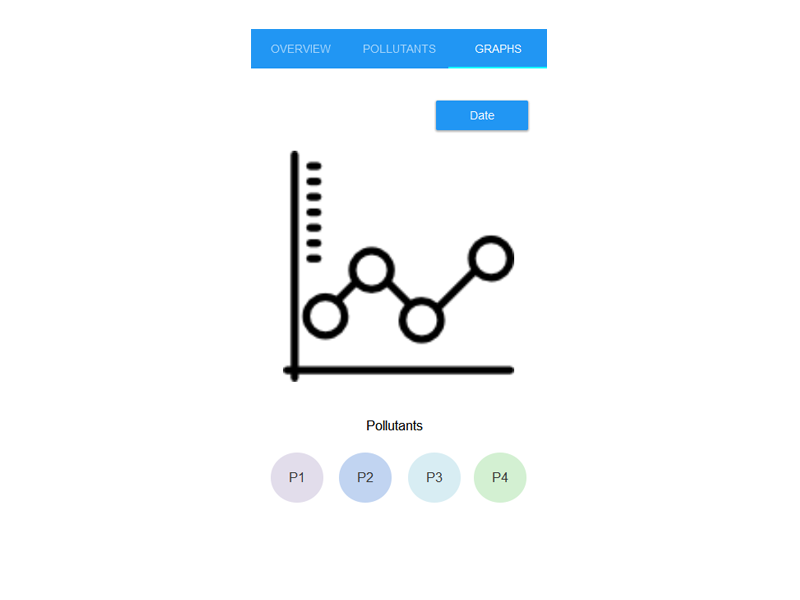
\includegraphics[scale=1]{images/prototype1_screen3.png}
\end{adjustbox}
  \caption[Third screen prototype]{Third screen prototype}
  \label{fig:android_material_design}
\end{figure}
